%%%%%%%%%%%%%%%%%%%%%%%%%%%%%%%%%%%%%%%%%%%%%%%%%%%%%%%%%%%%%%%%%%%%%%%%%%%%%%%%
\chapter{Анализ существующих решений}
%%%%%%%%%%%%%%%%%%%%%%%%%%%%%%%%%%%%%%%%%%%%%%%%%%%%%%%%%%%%%%%%%%%%%%%%%%%%%%%%

Наиболее известными инструментами, реализующими проверку моделей общего назначения, являются NuSMV и SPIN. Рассмотрим существующие графические интерфейсы пользователя для данных систем и оценим их по приведенным ниже критериям:

\begin{enumerate}
	\item \textit{Платформы} -- официально поддерживаемые программные платформы;
	\item \textit{Графическое построение модели} -- наличие графического редактора моделей;
	\item \textit{Визуализация контрпримера} -- наличие визуализации вывода NuSMV;
	\item \textit{Реализация} -- язык и технологии, используемые при реализации программы.
\end{enumerate}

\section{Графические интерфейсы пользователя для Spin}
	
В сегменте графических пользовательских интерфейсов для Spin представлены две программы: iSpin и jSpin. Рассмотрим их подробнее.

\subsection{iSpin}

iSpin – официально поддерживаемый сообществом Spin пакет, предоставляющий графический пользовательский интерфейс. Поддерживает все основные режимы работы. Имеет окно «Automata view», отображающее сгенерированный на основе описания модели конечный автомат. 

%Рис. Окно iSpin.

\begin{table}[ht]
	\caption{iSpin}\label{tab:ispin}
	\centering
	\begin{tabular}{|m{2.5 cm}|m{7.5 cm}|}
	\hline
	Платформы & Linux, Windows, Mac OS X \\
	\hline
	Графическое построение модели &Отсутствует \\
	\hline
	Визуализация контрпримера & Отсутствует \\
	\hline
	Реализация & Написан на языке Tcl с помощью библиотеки Tk.\\
	\hline
	\end{tabular}
\end{table}

\subsection{jSpin}

Программа iSpin разработана на языке Java. Программа состоит из есдинственного окна, состоящего из меню и трех текстовых полей:

\begin{enumerate}
	\item поле редактирования исходного кода Promela,
	\item поле отображения вывода Spin,
	\item поле отображения предупреждений компилятора.
\end{enumerate}

%Рис. Окно jSpin.

\begin{table}[ht]
	\caption{jSpin}\label{tab:jspin}
	\centering
	\begin{tabular}{|m{2.5 cm}|m{7.5 cm}|}
		\hline
		Платформы & Linux, Windows, Mac OS X \\
		\hline
		Графическое построение модели &Отсутствует \\
		\hline
		Визуализация контрпримера & Отсутствует \\
		\hline
		Реализация & Реализован с помощью языка Java.\\
		\hline
	\end{tabular}
\end{table}

\section{Графические интерфейсы пользователя для NuSMV}

В сегменте графических пользовательских интерфейсов для NuSMV представлены три программы: NuSMV GUI, gNuSMV и NuSeen.

\subsection{NuSMV GUI}

Программа разрабатывается непосредственно сообществом NuSMV, основывается на интерактивном режиме выполнения и предоставляет стандартные возможности редактирования исходного текста описаний моделей *.smv, редактирования спецификаций с помощью инспектора формул темпоральных логик CTL/LTL, а также предоставления вывода NuSMV в текстовом формате. Использует устаревшую версию NuSMV 1.

%Рис. Окно редактирования исходного кода NuSMV GUI

%Рис. Окно редактирования спецификаций NuSMV GUI

\begin{table}[ht]
	\caption{NuSMV GUI}\label{tab:nusmv_gui}
	\centering
	\begin{tabular}{|m{2.5 cm}|m{7.5 cm}|}
		\hline
		Платформы & Linux, Windows, Mac OS X \\
		\hline
		Графическое построение модели &Отсутствует \\
		\hline
		Визуализация контрпримера & Отсутствует \\
		\hline
		Реализация & Основан на Qt Jambi – библиотеке, представляющей собой Java-обёртку для Qt-компонентов.\\
		\hline
	\end{tabular}
\end{table}

\subsection{gNuSMV}

Данный проект находится в разработке, но для пользователей доступна snapshot версия программы. Главным отличием от NuSMV GUI является использование последней мажорной версии NuSMV 2.1. 

%Рис. Окно редактирования исходного кода gNuSMV.

%Рис. Окно редактирования спецификаций gNuSMV.


\begin{table}[ht]
	\caption{gNuSMV}\label{tab:gnusmv}
	\centering
	\begin{tabular}{|m{2.5 cm}|m{7.5 cm}|}
		\hline
		Платформы & Linux, Windows \\
		\hline
		Графическое построение модели &Отсутствует \\
		\hline
		Визуализация контрпримера & Отсутствует \\
		\hline
		Реализация & Основывается на pygtk2 – библиотеке для языка python, позволяющей строить графические приложения с помощью библиотеки GTK+2.\\
		\hline
	\end{tabular}
\end{table}

\subsection{NuSeen}

В отличие от вышерассмотренных графических интерфейсов, являющихся самостоятельными приложениями, NuSeen основан на интегрированной среде разработки Eclipse. Отличительной особенностью является построение графов зависимостей переменных и графов зависимостей жестко соединенных наборов переменных (SCV – Strongly Connected Variables set). Поддерживается визуализация контрпримера.

\begin{figure}[htbp]
	\centering
	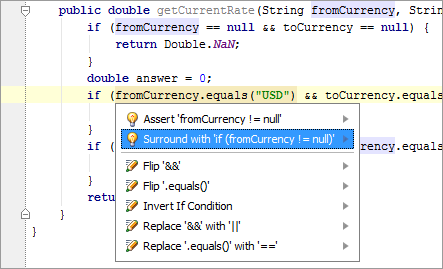
\includegraphics[width=0.8\textwidth]{fig/code_analysis_bugs.png}
	\caption{Предупреждение от статического анализатора в IntelliJ IDEA и всплывающее меню Quick Fix}%
	\label{fig:idea}
\end{figure}

%Рис. Окно визуализации контрпримера NuSeen.

%Рис. Пример графа зависимостей переменных NuSeen.


\begin{table}[ht]
	\caption{NuSeen}\label{tab:nuseen}
	\centering
	\begin{tabular}{|m{2.5 cm}|m{7.5 cm}|}
		\hline
		Платформы & Linux, Windows, Mac OS X \\
		\hline
		Графическое построение модели & Отсутствует \\
		\hline
		Визуализация контрпримера & Отсутствует \\
		\hline
		Реализация & Основан на интегрированной среде разработки Eclipse.\\
		\hline
	\end{tabular}
\end{table}

\section{Вывод}

Все рассмотренные выше реализации графических пользовательских интерфейсов для верификаторов общего назначения имеют схожие минусы:
\begin{itemize}
	\item Нет реализации графического редактора верифицируемых моделей;
	\item Визуализация контрпримера реализована только в NuSeen, но на очень примитивном уровне;
	\item Для проверки модели необходима установка ПО и зависимых пакетов;
\end{itemize}
